% (c)~2019 Daniele Zambelli daniele.zambelli@gmail.com % (c)~2019 
% Andrea Sellaroli

% \input{\folder finanziaria_grafici.tex}

\chapter{Matematica finanziaria}

La matematica finanziaria è quella parte della matematica applicata che si 
occupa degli scambi di somme di denaro disponibili in tempi diversi.

Se presto una certa somma di denaro (\textbf{capitale}) per un anno, io non 
potrò più usare quel denaro, e mi aspetto di essere remunerato per ciò. 
Specularmente, se uso del denaro che non possiedo, dovrò pagare una certa somma 
per il prestito ricevuto. 

L'\textbf{interesse} è il compenso che spetta a colui che concede in prestito un 
capitale, rinunciando per un certo periodo di tempo al suo utilizzo. 

Il \textbf{tasso di interesse} viene espresso come una percentuale per un dato 
periodo di tempo e indica quanta parte della somma prestata (detta capitale 
inziale) debba essere corrisposta come interesse al termine del tempo 
considerato. Il debitore, infatti, ricevendo una somma di denaro, si impegna a 
pagare una somma superiore a quella ricevuta. 

\begin{exrig} \begin{esempio} Deposito in banca 3000 € \,e, un anno dopo, ne 
ritiro 3150 €. Gli interessi sono dati dalla differenza tra il capitale finale e 
il capitale iniziale e quindi sono 150 €. Il tasso di interesse è la percentuale 
degli interessi sul capitale iniziale e quindi $$ i = \dfrac{150}{3000} = 0,05 
$$ ovvero il 5\%. \`{E} importante notare che tale tasso di interesse è 
strettamente riferito al periodo di tempo (in questo caso un anno). Pertanto è 
più corretto affermare che il tasso di interesse è del 5\% annuo. \end{esempio}

\begin{esempio} Ho acquistato un nuovo computer di 700 € sfruttando un offerta 
che mi permette di pagarlo tra un anno, pagando un interesse del 3\%. 
L'interesse che dovrò pagare sarà di $700 \cdot 0,03 = 21$ € ed alla fine il 
computer mi costerà 721 €. Per calcolare quantro dovro pagare il computer alla 
fine quindi devo fare $700+700\cdot0,03$. Un modo più rapido per calcolarlo è 
quello di moltiplicare 700 per 1,03, infatti $700(1+0,03)=700\cdot1,03=721$ 
\end{esempio}

\end{exrig}

\vspace{.4cm}

I tassi d'interesse sono caratterizzati dal regime di capitalizzazione degli 
interessi, che può essere semplice o composto. Se la durata del prestito è 
superiore al periodo di tempo per cui l'interesse viene conteggiato (ad esempio 
un tasso di interesse annuo calcolato per 4 anni), si parla di tasso di 
interesse composto, perché vengono conteggiati nel calcolo dell'interesse finale 
anche gli interessi parziali già maturati per ogni periodo.

\section{Capitalizzazione semplice} L'interesse viene detto semplice quando è 
proporzionale al capitale e al tempo. Ovvero gli interessi, maturati da un dato 
capitale nel periodo di tempo considerato, non vengono aggiunti al capitale che 
li ha prodotti (capitalizzazione) e, quindi, non maturano a loro volta 
interessi. Indichiamo:

\begin{itemize} \item \textbf{C} il capitale iniziale; \item \textbf{i} il tasso 
di interesse periodale (in genere tasso unitario annuo, ma può essere mensile, 
trimestrale...); \item \textbf{t} durata temporale dell'operazione, espressa in 
numero di periodi (in genere anni); \item \textbf{M} il capitale finale, detto 
anche montante, pari alla somma di capitale iniziale più gli interessi maturati. 
\end{itemize}

All'istante iniziale ($t=0$) possiamo dire che il montante coincide col capitale 
$$ M_{0}=C $$ Dopo un periodo di tempo ($t=1$), il montante sarà dato dal 
capitale più l'interesse. $$ M_{1}=M_{0} +iC = C + iC $$ Analogamente dopo 2, 3 
e 4 periodi di tempo il capitale sarà dato da $$ M_{2}=M_{1} +iC = (C + iC) +iC 
= C +2iC$$ $$ M_{3}=M_{2} +iC = (C + 2iC) +iC = C +3iC$$ $$ M_{4}=M_{3} +iC = (C 
+ 3iC) +iC = C +4iC$$ In generale possiamo calcolare il montante per il periodo 
successivo con la formula: $$ M_{t}=M_{t-1}+iC=C(1+t\cdot i) $$ 
\begin{definizione}[Capitalizzazione semplice] $$ M_{t}=C(1+t\cdot i) $$ 
\end{definizione}

\begin{exrig} \begin{esempio} Una persona deposita 5000 € in banca al tasso di 
interesse annuo del 5\%. Dopo 4 anni preleva la somma e la reinveste al tasso 
annuo del 6\%. Dopo altri 5 anni e 9 mesi di che cifra dispone? Il capitale 
iniziale è di 5000 € ed applicando la formula di capitalizzazione semplice 
otteniamo che il montante dopo 4 anni è

$$M_4 = 5000(1+4\cdot0,05) = 6000$$ Quando questa cifra viene prelevata e 
reinvestita possiamo considerarla come il nuovo capitale iniziale. La durata 
temporale, in questo caso, è espressa in anni e in mesi. Convertendola in anni 
otteniamo $t = 5 +\frac{9}{12} = 5,75$ e quindi

$$M_{5,75} = 6000(1+5,75\cdot0,06) = 8070$$ \end{esempio} \end{exrig}

\section{Capitalizzazione composta}

L'interesse viene detto composto quando, invece di essere pagato o riscosso, è 
aggiunto al capitale iniziale che lo ha prodotto. Questo comporta che, alla 
maturazione degli interessi, il montante verrà riutilizzato come capitale 
iniziale per il periodo successivo. Quindi anche l'interesse stesso produce a 
sua volta interesse.

In questo caso quindi gli interessi si sommano al capitale iniziale che li ha 
prodotti al termine di ogni periodo. Analogamente a prima il montante iniziale 
coincide col capitale $$ M_{0}=C $$ Dopo un periodo il montante sarà dato dal 
capitale più l'interesse $$M_{1}=C+iC=C(1+i)$$ Calcoliamo adesso l'interesse su 
tutto il montante $M_1$ e troviamo $$M_{2}=M_1+iM_1=M_1(1+i)=C(1+i)^2$$ 
$$M_{3}=M_2+iM_2=M_2(1+i)=C(1+i)^3$$ ed in generale risulta $$M_{t}=M_{t-1}(1+i) 
= C(1+i)^{t-1}(1+i)=C(1+i)^{t}$$

\begin{definizione}[Capitalizzazione composta] $$ M_{t}=C(1+i)^t $$ 
\end{definizione}

In generale il periodo considerato è l'anno. Spesso però vengono considerati 
anche gli interessi che maturano $t$ volte durante l'anno, ma sempre in periodi 
definiti. In genere viene definito un tasso annuo nominale $i$ al quale 
corrisponde un tasso convertibile $i_c$ dato da

$\ i_c = \frac{i}{t}$.

Per il calcolo del montante si applica la stessa formula impiegata per 
l'interesse composto $\ M_n = C (1+i_c)^{nt} = C 
\left(1+\frac{i}{t}\right)^{nt}$.

dove $i_c$ è l'interesse convertibile e $nt$ indica il numero di volte in cui 
l'interesse convertibile matura nell'intero periodo.

\begin{exrig} \begin{esempio} Un ``amico'', 20 anni fa, mi ha prestato 500 € al 
tasso di interesse del 9\% in regime di capitalizzazione composta. Per capire 
quanto gli devo restituire oggi posso usare la formula per la capitalizzazione 
composta. $$M_{20} = 500(1+0,09)^{20} = 2802,21$$ Come si nota subito in 20 anni 
la cifra iniziale è più che quintuplicata. In effetti il tasso del 9 \% è un 
tasso da usura. \end{esempio} \begin{esempio} Un capitale di 10000 € è stato 
investito per un periodi di 30 mesi al tasso trimestrale convertibile dell'1\% . 
Considerando che ci sono 4 trimestri in un anno, il tasso annuo nominale risulta 
quindi $$i=i_c\cdot t=1\cdot 4=4\%$$ Dopo 30 mesi, ovvero 10 trimestri, il 
montante risulta $$M=10000(1+0,01)^{10}=11046,22$$ \end{esempio} \end{exrig}

\subsection{Scindibilità finanziaria} Si dice che un regime finanziario è 
\textbf{scindibile} se il montante di un'operazione finanziaria dipende solo 
dalla durata e non da eventuali operazioni di disinvestimento ed investimento 
intermedie (ossia da operazioni di capitalizzazione intermedie). La 
capitalizzazione semplice non è scindibile nel tempo, infatti se investo 3000 € 
per 5 anni con un tasso di interesse $i=0,08$ ottengo 
$$3000(1+5\cdot0,08)=4200$$ mentre se li disinvesto dopo 2 anni e li reinvesto 
immediatamente per altri 3 ottengo $$3000(1+2\cdot0,08)=3480$$ e poi 
$$3480(1+3\cdot0,08)=4315,2$$ che sono cifre diverse. Lo stesso problema, con la 
capitalizzazione composta, risulta $$3000(1+cdot0,08)^5=4408$$ se aspetto 5 anni 
oppure $$3000(1+0,08)^2=3499$$ e poi $$3499(1+0,08)^3=4408$$ se invece 
disinvesto dopo 2 anni e reinvesto per 3. Come si vede in questo caso le due 
cifre sono uguali. Questo è un fatto più generale (dipende dalle proprietà delle 
potenze) e quindi la capitalizzazione composta è scindibile. Per questa 
importante proprietà, nel seguito, utilizzeremo sempre la capitalizzazione 
composta. \begin{comment} \section{Capitalizzazione composta continua}

In questo caso gli interessi si sommano al capitale che li ha prodotti ad ogni 
istante. Il tasso d'interesse composto a capitalizzazione continua ha 
applicazioni soprattutto teoriche, nella matematica finanziaria; sebbene sia 
rilevante nelle applicazioni relative alle più semplici operazioni finanziarie, 
è ad esempio ampiamente utilizzato nelle formule di valutazione di operazioni 
finanziarie complesse, come nella valutazione delle opzioni.

L'interesse in capitalizzazione continua può essere giustificato come segue. Si 
consideri un tasso annuale $i$, e si supponga di suddividere l'anno in $t$ 
periodi, al termine di ciascuno dei quali viene corrisposta una frazione 
dell'interesse relativo all'intero anno pari a $\frac{i}{t}$, che viene 
immediatamente reinvestita. A partire da un capitale iniziale $C$, il montante 
al termine di $n$ anni sarà allora \\[4pt] $\ 
M_n=C\left(1+\frac{i}{t}\right)^{nt}$ \\[4pt] Passando al limite per $t$ che 
tende a infinito, si ha il caso in cui un flusso continuo di pagamenti viene 
reinvestito in maniera continua; il montante sarà dato da \\[4pt] $$\ M_n = 
\lim_{t\to\infty} C\left(1+\frac{i}{t}\right)^{nt} = Ce^{in}$$, \\[4pt] 
ricorrendo al limite notevole che definisce il numero di Nepero $e$.

\subsection{Tassi equivalenti}

Chiamiamo \emph{tassi equivalenti} due tassi d'interesse che, applicati allo 
stesso capitale, producono lo stesso montante (ovviamente in tempi diversi). Per 
determinare la relazione tra due tassi unitari ad interesse composto $i_{c1}$ e 
$i_{c2}$ è sufficiente uguagliare i montanti che sono prodotti da periodi di 
tempo $t_1$ e $t_2$ differenti $$M = C(1+i_{c1})^{t_1} = C(1+i_{c2})^{t_2}$$. Da 
questa si ottengono le relazioni: $$i_{c1} = (1+i_{c2})^\frac{t_2}{t_1}-1 
\hspace{1cm} i_{c2} = (1+i_{c1})^\frac{t_1}{t_2}-1$$ \end{comment} 
\section{Trasporto di capitali nel tempo} Da quanto detto sulla capitalizzazione 
semplice e composta dovrebbe risultare abbastanza chiaro che non è possibile 
sommare, sottrarre o confrontare valori di denaro differiti nel tempo. Per prima 
cosa infatti è necessario riferirli allo stesso momento temporale. Abbiamo già 
visto che un capitale, trasportato in avanti nel tempo, diventa un montante 
(somma del capitale iniziale e degli interessi) e tale processo si chiama 
capitalizzazione. All'inverso, un capitale portato indietro nel tempo si chiama 
valore attuale (o valore scontato) e il processo si definisce attualizzazione (o 
sconto). 


\subsection{Capitalizzazione} Per trasportare avanti nel tempo un capitale in un 
regime di capitalizzazione composta la formula è già stata vista e risulta 
$M=C(1+i)^n$ dove $n$ indica il numero di periodo (nella figura qui sotto, ad 
esempio, $n=5$).

\begin{figure}[htp] \centering 
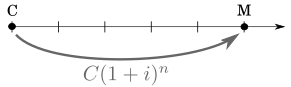
\includegraphics[scale=.60]{img/capitalizzazione.png} \end{figure}


\subsection{Attualizzazione} Trasportare un capitale indietro nel tempo di $n$ 
periodi, prevede di calcolare qual è la cifra di partenza, detta $valore 
attuale$ (o sconto) per cui, dopo $n$ intervalli, si è arrivati a quel capitale. 
Il valore attuale, quindi, dopo $n$ invervalli, viene attualizzato e diventa il 
capitale di partenza, in formule $C=V(1+i)^n$. \begin{figure}[htp] \centering 
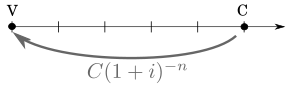
\includegraphics[scale=.60]{img/attualizzazione.png} \end{figure}

Invertendo la formula risulta $V=\dfrac{C}{(1+i)^n}$ e ricordando le proprietà 
delle potenze\footnote{ovvero che $\dfrac{1}{x^n}=x^{-n}$} risulta



\begin{definizione}[Attualizzazione] $$ V=C(1+i)^{-n}$$ \end{definizione} 
\begin{exrig} \begin{esempio} Voglio sommare 2000 € che ho ricevuto 2 anni fa, 
1000 € euro ricevuti oggi e 1600 € che riceverò tra 3 anni, utilizzando un tasso 
di interesse $i=0,05$. Trasporto tutti i capitali alla data attuale. 
\begin{figure}[htp] \centering 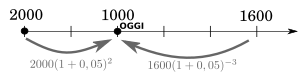
\includegraphics[scale=.60]{img/esempio.png} 
\end{figure} \begin{itemize} \item I 2000 € vanno capitalizzati e quindi risulta 
$M=2000(1+0,05)^2=2205$ \item I 1000 € sono già alla data attuale \item I 1600 € 
vanno attualizzati e risulta $M=1600(1+0,05)^{-3}=1382$ \end{itemize} La somma 
totale alla data odierna è quindi $2205+1000+1382=4587$ \end{esempio} 
\end{exrig}

\'E interessante notare che per frazioni dell'anno si possono usare esponenti 
frazionari, ad esempio se devo trasportare in avanti di 3 mesi (che sono 
$\frac{3}{12}$ di anno) un capitale al tasso di interesse annuo del 5\% posso 
fare $M=C(1+0,05)^{\frac{3}{12}}$





\section{Intermezzo matematico: la serie geometrica} Per il seguito è necessario 
imparare a sommare le prime $n$ potenze di un numero fissato $q$, detta 
$ragione$. In alcuni casi posso farlo direttamente, ad esempio la somma 
$2^0+2^2+2^2+2^3+2^4=31$ ma se devo fare $3^0+3^1+3^2+\dots+3^{42}$ devo 
sviluppare un altro metodo. Indichiamo con $S$ la somma delle prime $n$ potenze 
di un numero generico $q$ $$ S= 1+q+q^2+q^3+\dots + q^{n-1}+q^n$$ moltiplichiamo 
da entrambi i lati per $q-1$ $$ S(q-1)= (1+q+q^2+q^3+\dots + q^{n-1}+q^n)(q-1)$$ 
e quindi sviluppando il prodotto tra polinomio e binomio risulta $$ S(q-1)= 
q+q^2+q^3+q^4+\dots + q^{n}+q^{n+1}-1-q-q^2-q^3-\dots - q^{n-1}-q^n$$ la maggior 
parte dei termini si semplifica compresi i termini sottointesi dai puntini e 
risulta $$ S(q-1)= \cancel{q}+\cancel{q^2}+\cancel{q^3}+\cancel{q^4}+\dots + 
\cancel{q^n}+q^{n+1}-1-\cancel{q}-\cancel{q^2}-\cancel{q^3}-\dots - 
\cancel{q^{n-1}}-\cancel{q^n}$$ quindi $$S(q-1)=q^{n+1}-1 $$ e semplificando 
risulta \begin{definizione}[Serie geometrica] $$ 1+q+q^2+q^3+\dots + 
q^{n-1}+q^n=\dfrac{q^{n+1}-1}{q-1} $$ \end{definizione}

\begin{exrig} \begin{esempio} Si narra che l’inventore del gioco degli scacchi 
chiedesse di essere compensato con chicchi di grano: un chicco sulla prima 
casella, due sulla seconda, quattro sulla terza e così via, sempre raddoppiando 
il numero dei chicchi, fino alla sessantaquattresima casella. Assumendo che 1000 
chicchi pesino circa 38 g, calcola il peso in tonnellate della quantità di grano 
pretesa dall’inventore.

Come prima cosa sommiano le prime $64$ potenze di due; ricordandosi di contare 
anche $2^0=1$.

$$ 1+2+2^2+2^3+\dots + 2^63=\dfrac{2^{63+1}-1}{2-1}=2^{64}-1=1,84 \cdot10^{19}$$

Se 1000 chicchi di grano pesano 38 g, allora il peso totale dei chicchi sulla 
scacchiera vale  $7.00976\cdot10^{17} g$ ossia $7.00976\cdot10^{14} kg = 
7.00976\cdot10^{11}$ tonnellate. 

\end{esempio} \end{exrig}

\section{Rendite} Una rendita finanziaria è una successione di importi, chiamate 
rate, da riscuotere (o da pagare) in epoche differenti, chiamate scadenze, ad 
intervalli di tempo determinati. Per semplicità considereremo nel seguito 
intervalli di tempo di durata costante e rate costanti (ovvero tutte uguali).

\begin{exrig} \begin{esempio} \label{nonna} Una nonna versa alla nipote 500 € 
per ogni compleanno dalla prima candelina fino al diciottesimo. Alla maggiore 
età la nipote ritirerà un montante dato dalla somma delle 18 rate (9000 €) più 
gli interessi, che saranno dati dalla capitalizzazione di 17 periodi per i primi 
500 euro, di 16 periodi per i 500 euro versati al secondo compleanno e così via 
fino ai 500 euro versati al diciottesimo su cui non saranno maturati interessi. 
\end{esempio} \end{exrig}

Esistono diversi tipi di rendite, che possono essere caratterizzate da diversi 
fattori

\begin{itemize} \item La \textbf{rata}, cioò l'importo da pagare ad ogni 
periodo, che può essere costante o variabile nel tempo. Per semplicità, nel 
seguito, ci occuperemo solo di \textit{rate costanti}. Indicheremo la rata con 
$R$ \item Il \textbf{numero} di rate da pagare che consideremo sempre finito e 
indicheremo con $n$. Esistono però anche rendite (dette perpetue o vitalizie) in 
cui $n$ non è finito o non è determinato fin dall'inizio. \item Il 
\textbf{periodo} ovvero l'intervallo di tempo che c'è tra una rata e l'altra. 
Generalmente tale intervallo sarà annuale, ma potrebbe essere anche mensile, 
trimestrale o altro. Il tasso di interesse $i$ deve essere riferito al periodo. 
\item La \textbf{decorrenza} che indica da quando può essere pagata (o riscossa) 
la prima rata. Noi ci occuperemo solo di rendite \textit{immediate}, ovvero 
quelle in cui si inizia a pagare nel primo periodo, ma esistono anche le rendite 
differite, in cui si paga o riscuote la prima rata dopo un certo numero di 
periodi (un esempio è la pensione). \item La \textbf{scadenza} della rata ovvero 
se si paga all'inizio del periodo (\textit{rendita anticipata}) o alla fine del 
periodo (\textit{rendita posticipata}). Ad esempio una rendita annuale è 
anticipata se pago le rate al 1 gennaio e posticipata se le pago il 31 dicembre. 
\end{itemize}


Per capire il meccanismo matematico che c'è dietro alle rendite analizzeremo 
soltanto alcune rendite particolari ovvero le rendite immediate con il numero 
delle rate totali finito e le scadenze separate da intervalli di tempo uguale. 
Studieremo queste rendite nel caso in cui siano anticipate o posticipate. 

\subsection{Rendite immediate posticipate a rate costanti} Nelle rendite 
immediate posticipate a rate costanti abbiamo \begin{itemize} \item La 
\textbf{rata} $R$ che è costante e pagata alla fine di ogni periodo \item Il 
\textbf{numero} di periodi $n$ fissato (e la durata dei periodi costante) \item 
Il \textbf{tasso di interesse} $i$ riferito alla durata del periodo 
\end{itemize} Vediamo adesso come possiamo calcolare il \textbf{montante} $M$. 
Si tratta di capitalizzare (ovvero trasportare avanti nel tempo) ogni singola 
rata. \begin{figure}[htp] \centering 
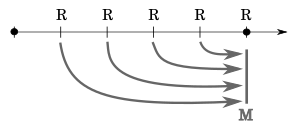
\includegraphics[scale=1]{img/posticipata.png}

\end{figure}

Nella figura abbiamo $n=5$ anche se la prima rata viene pagata alla fine del 
primo periodo; dovrà quindi essere trasportata in avanti di 4 periodi, in 
formule $M=R(1+i)^4$. Per lo stesso motivo, la seconda rata dovrà essere portata 
in avanti di 3 periodi ovvero $M=R(1+i)^3$. La penultima rata deve essere 
portata avanti solo di un periodo, quindi $M=R(1+i)^1$ mentre l'ultima rata è 
già alla data in cui viene calcolato il montante, quindi $R$ Il montante sarà 
quindi dato dalla somma di tutte le rate capitalizzate ovvero

$$M=R+R(1+i)+R(1+i)^2+R(1+i)^3+R(1+i)^4$$

nel caso di un numero di rate generico $n$ tale formula diventa

$$M=R+R(1+i)+R(1+i)^2+\dots+R(1+i)^{n-1}$$ e, raccogliendo $R$, risulta

$$M=R\big(1+(1+i)+(1+i)^2+\dots+(1+i)^{n-1}\big)$$ che è una serie geometria di 
ragione $(1+i)$ e quindi

$$M=R\dfrac{(1+i)^{(n-1+1)}-1}{1+i-1} $$ che semplificando risulta

\begin{definizione}[Montante di rendita posticipata] $$ M=R\dfrac{(1+i)^n-1}{i} 
$$ \end{definizione}

Per trovare il valore attuale di questo montante basta attualizzarlo di $n$ 
periodi ovvero $$V=M(1+i)^{-n}$$ che sostituendo con il valore del montante per 
una rendita posticipata risulta

 $$V=R\dfrac{(1+i)^n-1}{i}(1+i)^{-n}$$ e applicando le proprietà delle potenze 
risulta


\begin{definizione}[Valore attuale di rendita posticipata] $$ 
V=R\dfrac{1-(1+i)^{-n}}{i} $$ \end{definizione}

\begin{exrig} \begin{esempio} Rivediamo l'esempio \ref{nonna} (nonna e nipote). 
Abbiamo $R=500$ ed $n=18$. Supponiamo un tasso d'interesse $i=0,02$, possiamo 
calcolare il montante

$$ M=500\dfrac{(1+0,02)^{18}-1}{0,02}=10\;706,16 $$

ed il valore attuale

$$ V=500\dfrac{1-(1+0,02)^{-18}}{0,02}=7\;496,02 $$ \end{esempio} \end{exrig}

\subsection{Rendite immediate anticipate a rate costanti} Nel caso della rendita 
anticipata la rata viene pagata all'inizio del periodo. Senza dover ripetere il 
procedimento della serie geometrica posso immaginare una rendita anticipata come 
una rendita posticipata in cui ogni rata non valgone $R$ ma $R(1+i)$. Infatti la 
differenza tra le due sta nel fatto che ogni rata viene trasportata avanti di un 
periodo, maturando un'interesse di $i$. \begin{figure}[htp] \centering 
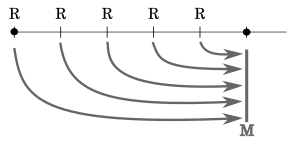
\includegraphics[scale=1]{img/anticipata.png}

\end{figure} Montante e valore attuale di una rendita anticipata risultano 
quindi: \begin{definizione}[Montante di rendita anticipata] $$ 
M=R(1+i)\dfrac{(1+i)^n-1}{i} $$ \end{definizione}


\begin{definizione}[Valore attuale di rendita anticipata] $$ 
V=R(1+i)\dfrac{1-(1+i)^{-n}}{i} $$ \end{definizione}

\section{Ammortamenti} In finanza, per ammortamento si intende il processo con 
il quale il debitore restituisce il capitale preso a prestito e gli interessi 
maturati sul debito.

Il capitale mutuato S viene diviso in quote di capitale a cui vengono aggiunti 
gli interessi, la somma dà la rata di ammortamento da corrispondere in epoche 
solitamente equintervallate.

Le rate di ammortamento comprendono una quota di capitale e una di interessi: 
$$R=Q+I$$

Esistono diversi tipi di ammortamenti (a capitale costante, a rate costanti, a 
due tassi); per il seguito ci occuperemo di quello a \textbf{rate costanti} 
detto ammortamento alla francese.

L'ammortamento francese prevede che le rate siano posticipate e che la somma 
ricevuta dal debitore all'inizio sia il valore attuale di una rendita a rate 
costanti. Ciascuna rata è comprensiva di parte del capitale (quota capitale) ed 
i relativi interessi (quota interessi) calcolati sul capitale residuo non ancora 
restituito (debito residuo). 

Per calcolare il valore della rata, noto capitale inziale, numero di periodi e 
tasso d'interesse, basta applicare la formula inversa al valore attuale di una 
rendita posticipata 

\begin{definizione}[Rata] $$ R=C\dfrac{i}{1-(1+i)^{-n}}$$ \end{definizione}

\begin{exrig} \begin{esempio} Ho chiesto un prestito di $20\;000$ euro che 
voglio restiture in $10$ anni. Se il tasso di interesse annuo è del $3,5\%$, 
quanto dovrò pagare ad ogni rata?

Utilizzando la formula risulta: $$ 
R=20\;000\dfrac{0,035}{1-(1,035)^{-10}}=2\;404,83$$ Quindi devo pagare 10 rate 
annue da circa 2405 €. \end{esempio} \end{exrig}

Come detto in precedenza ogni rata è composta da una quota di capitale e una 
quota di interessi. Visto che il debito residuo diminuscie ad ogni periodo la 
quota di interessi diminuirà sempre, e di conseguenza, essendo le rate costanti, 
aumenterà la quota di capitale.

\subsection{Piano di ammortamento} Vediamo adesso come stendere un piano di 
ammortamento (alla francese), ovvero un programma di estinzione del debito. Per 
prima cosa si calcola il valore della rata, che sarà costante. Poi si costruisce 
una tabella con una riga per ogni periodo (più una riga per il momento iniziale 
o periodo $0$) e 6 colonne che saranno \begin{itemize} \item il periodo di 
riferimento \item \textbf{R}: il valore della rata (che nel nostro caso sarà 
costante) \item \textbf{Q}: la quota di capitale della rata \item \textbf{I}: la 
quota di interesse della rata \item \textbf{D}: il debito residuo \item 
\textbf{E}: il debito estinto \end{itemize} Per ogni periodo $k$ la somma tra 
capitale e interesse deve corrispondere con il valore della rata, in formule: 
$$R=Q_k+I_k$$ Inoltre la somma tra debito estinto e residuo in ogni periodo $k$ 
dovrà equivalere al capitale iniziale. $$C=D_k+E_k$$ Il principio con cui si 
costruisce il piano di ammortamento alla francese è che la quota di interesse 
per ogni periodo è calcolata sul debito residuo al periodo precedente. In 
formule $$I_{k+1}=i\cdot D_k$$ Vediamo con un esempio come fare operativamente

\begin{exrig} \begin{esempio} Stendere un piano di ammortamento per un prestito 
di $5\;000$ euro da restiture in $4$ anni ad un tasso di interesse annuo del 
$10\%$.

Per prima cosa calcoliamo il valore della rata $$ 
R=5\;000\dfrac{0,1}{1-(1,1)^{-4}}=1\;577,35$$

Iniziamo a stendere la tabella con quello che conosciamo al momento iniziale. I 
valori delle rate sono sempre costantemente uguali a $1\;577,35$ (tranne che nel 
periodo 0 perché è posticipata), il debito residuo coincide col capitale 
iniziale ed il debito estinto è zero


\begin{tabular}{c|c|c|c|c|c} \hline periodo & rata & quota capitale & quota 
interesse & debito residuo & debito estinto\\ \hline & R & Q & I & D & E\\ 
\hline 0 &  &  &  & $5000$ & $0$\\ 1 & $1\;577,35$ &  &  &  & \\ 2 & $1\;577,35$ 
&  &  &  & \\ 3 & $1\;577,35$ &  &  &  & \\ 4 & $1\;577,35$ &  &  &  & \\ \hline 
\end{tabular} La prima rata è formata da una quota di capitale ed una di 
interesse. La quota di interesse è calcolata sul debito residuo quindi 
$I_1=i\cdot D_0=0,1\cdot 5000=500$. La quota capitale si calcola ricordando che 
la somma tra quota capitale e interesse è la rata: 
$Q_1=R-I_1=1577,35-500=1077,35$. A questo punto ho rimborsato una parte del 
capitale, e quindi il debito residuo sarà dato dal debito al periodo precedente 
meno la quota di capitale pagata ovvero $D_1=D_0-Q_1=5000-1077,35=3922,65$. Per 
calcolare la parte di debito estinto basta ricordare che $C=D_k+E_k$ e quindi 
$E_1=C-D_1=5000-3922,65=1577,35$. Inserendo i dati in tabella risulta:

\begin{tabular}{c|c|c|c|c|c} \hline periodo & rata & quota capitale & quota 
interesse & debito residuo & debito estinto\\ \hline & R & Q & I & D & E\\ 
\hline 0 &  &  &  & $5000$ & $0$\\ 1 & $1\;577,35$ & $1\;077,35$ & $500$ & 
$3\;922,65$ & $1\;577,35$\\ 2 & $1\;577,35$ &  &  &  & \\ 3 & $1\;577,35$ &  &  
&  & \\ 4 & $1\;577,35$ &  &  &  & \\ \hline \end{tabular} Adesso per calcolare 
la quota di interesse nella seconda rata si utilizzerà il debito residuo del 
primo periodo ovvero $3\;922,65$ e si ripeteranno gli stessi calcoli. Alla fine 
il piano di ammortamento completo deve risultare:


\begin{tabular}{c|c|c|c|c|c} \hline periodo & rata & quota capitale & quota 
interesse & debito residuo & debito estinto\\ \hline & R & Q & I & D & E\\ 
\hline 0 &  &  &  & $5000$ & $0$\\ 1 & $1\;577,35$ & $1\;077,35$ & $500$ & 
$3\;922,65$ & $1\;577,35$\\ 2 & $1\;577,35$ & $1\;185,09$& $392,26$ & 
$2\;737,56$ & $2\;262,44$\\ 3 & $1\;577,35$ & $1\;303,60$ & $273,76$ & 
$1\;433,96$ & $3\;566,04$\\ 4 & $1\;577,35$ & $1\;433,96$ & $143,40$ & $0$ & 
$5\;000,00$\\ \hline \end{tabular} Come si può vedere la parte di interessi 
scende ad ogni rata ed aumenta la quota di capitale. Alla fine il debito residuo 
deve essere 0 e il debito estinto coincidere col capitale iniziale. 

\end{esempio} \end{exrig}

\begin{comment} 
\section{Esercizi}


\subsubsection{Capitalizzazione semplice}

\begin{esercizio} Calcola il valore incognito in un regime di capitalizzazione 
semplice \begin{enumeratea} \item $C = 2000$ \euro ;\quad $i = 0.02$ ;\quad $t = 
10$ anni;\quad $M=\;?$ \hfill [2400 \euro] \item $C = 5000$ \euro ;\quad $t = 5$ 
anni ;\quad $M = 5750$ \euro;\quad $i=\;?$ \hfill [$3 \%$] \item $M = 2530$ 
\euro ;\quad $i = 0.005$ ;\quad $t = 20$ anni;\quad $C=\;?$ \hfill [2300 \euro]

 \item $C = 60000$ \euro ;\quad $t = 6$ anni ;\quad $M = 63600$ \euro;\quad 
$i=\;?$ \hfill [$1 \%$]

 \item $C = 3000$ \euro ;\quad $i = 0,02$ ;\quad $t = 3$ mesi;\quad $M=\;?$ 
\hfill [3015 \euro]

 \end{enumeratea} \end{esercizio}


\begin{esercizio} Risolvi i seguenti problemi: \begin{enumeratea} \item Ho 
investito 15000 \euro\, in regime di capitalizzazione semplice per 3 anni a un 
tasso d'interesse del 5\% annuo. Quale interesse ho maturato?\hfill [2250 \euro] 
\item Cinque anni fa ho investito un certo capitale in regime di 
capitalizzazione composta al 3\% annuo. Oggi ho ritirato 12995 \euro. Quanti 
soldi avevo investito?\hfill [11300 \euro] \item Vengono investiti, in regime di 
capitalizzazione composta, 50000 \euro\; per 10 anni. Per ottenere un interesse 
di 1000 euro, a quale tasso d'interesse si deve investire tale somma?\hfill 
[0,02 \%] \end{enumeratea} \end{esercizio}

\subsection{Capitalizzazione composta} \begin{esercizio} Calcola il valore 
incognito in un regime di capitalizzazione composta \begin{enumeratea} \item $C 
= 2000$ \euro ;\quad $i = 0.02$ ;\quad $t = 10$ anni;\quad $M=\;?$ \item $C = 
5000$ \euro ;\quad $t = 5$ anni ;\quad $M = 5750$ \euro;\quad $i=\;?$ \item $M = 
2530$ \euro ;\quad $i = 0.005$ ;\quad $t = 20$ anni;\quad $C=\;?$ \hfill

 \item $C = 60000$ \euro ;\quad $t = 6$ anni ;\quad $M = 63600$ \euro;\quad 
$i=\;?$ \hfill 

 \item $C = 3000$ \euro ;\quad $i = 0,02$ ;\quad $t = 3$ mesi;\quad $M=\;?$ 
\hfill

 \end{enumeratea} \end{esercizio}


\begin{esercizio} Risolvi i seguenti problemi: \begin{enumeratea} \item Ho 
investito 15000 \euro\, in regime di capitalizzazione composta per 3 anni a un 
tasso d'interesse del 5\% annuo. Quale interesse ho maturato?\hfill \item Cinque 
anni fa ho investito un certo capitale in regime di capitalizzazione semplice al 
3\% annuo. Oggi ho ritirato 12995 \euro. Quanti soldi avevo investito?\hfill 
[11300 \euro] \item Vengono investiti, in regime di capitalizzazione semplice, 
50000 \euro\; per 10 anni. Per ottenere un interesse di 1000 euro, a quale tasso 
d'interesse si deve investire tale somma?\hfill [0,02 \%] \end{enumeratea} 
\end{esercizio}


\subsection{Trasporto di capitali nel tempo} \begin{esercizio} A seguito di 
alcuni investimenti dovrei riscuotere 7000 € tra 3 mesi, 10 000 € tra 6 mesi e 
8500 € tra un anno. Quanto posso riscuotere tra 5 mesi, al tasso annuo del 
2,5\%, \hfill[25 386,75] \end{esercizio}

\begin{esercizio} Acquisto oggi un'automobile e posso pagarla così. Oggi verso 
9500 €, tra 6 mesi verso 6000 € e tra 12 mesi verso 15700 €. Quanto vale 
l'automobile se viene applicato un tasso del 4\% annuo. \end{esercizio}


\subsection{Rendite} \begin{esercizio} Una persona vuole costituire una somma 
che gli consenta, fra 4 anni, di poter cambiare l'auto; per questo versa E 1350 
ogni quadrimestre a partire da oggi, ad un tasso annuo nominale convertibile 
quadrimestralmente del 6\%. Quale somma avrà a disposizione all'epoca stabilita? 
\hfill[18468,45] \end{esercizio} \begin{esercizio} Hai versato in banca E 8000 
alla fine di ogni anno e per 6 anni, al tasso annuo del 2,5\%. Se decidi di 
ritirare il capitale all'atto dell'ultimo versamento, di quale somma potrai 
disporre? \hfill[51101,89] \end{esercizio} \begin{esercizio} Fra 5 anni avremo 
bisogno di una somma 5200 € per restituire un prestito che ci è stato fatto. 
Decidiamo allora di depositare ogni anno, alla fine dell'anno, una somma che sia 
in grado di costituire questo capitale. Qual eÁ il valore di questa somma al 
tasso annuo del 4\%? \end{esercizio} \begin{esercizio} Una persona ha iniziato a 
versare 15 anni fa presso una banca 800 € all'anno ed ha proseguito i versamenti 
fino ad oggi; 4 anni fa, inoltre, ha depositato presso la stessa banca 9800 €. 
Per tutta la durata dell'operazione, la banca ha mantenuto costante il tasso 
d'interesse al 2,5\% annuo. Se oggi questa persona preleva 23000 € qual è il 
saldo del suo conto?

\end{esercizio}

\begin{esercizio} Riccardo sa che fra 6 anni avrà bisogno di 10000€ per 
festeggiare con un viaggio i suoi 25 anni di matrimonio. Calcola la rata annua 
anticipata al tasso dell'4,6\% annuo che Riccardo deve versare per poter 
costituire questo capitale. \end{esercizio} \begin{esercizio} Un appartamento 
viene affittato per un anno ad un canone mensile di 2 000 €. Volendo pagare 
anticipatamente l'intero ammontare del canone, quanto si deve versare al 
proprietario se la valutazione viene fatta al 2\% \end{esercizio}


\subsection{Ammortamenti} \begin{esercizio} Determina la rata di un mutuo per un 
capitale di $150\;000$, durata di $20$ anni e un tasso di interesse annuo del 
$4\%$ \end{esercizio} \begin{esercizio} Determina la rata di un prestito per un 
capitale di $4\;000$, durata di $5$ anni e un tasso di interesse annuo del $9\%$ 
\end{esercizio} \begin{esercizio} Determina la rata di un prestito per un 
capitale di $80\;000$, durata di $15$ anni e un tasso di interesse annuo del 
$1,5\%$ \end{esercizio} \begin{esercizio} Per un mutuo per $60\;000$ euro mi 
hanno proposto due opzioni: nella prima pago una rata di 530 € per 10 anni, 
nella seconda 380 € per 15 anni. Calcola i due tassi di interesse applicati. 
\end{esercizio}


\begin{esercizio} Stendi un piano di ammortamento per un prestito di $3\;500$, 
durata di $3$ anni e un tasso di interesse annuo del $2\%$ \end{esercizio} 
\begin{esercizio} Stendi un piano di ammortamento per un prestito di $42\;000$, 
durata di $6$ anni e un tasso di interesse annuo del $3\%$. Se decido di 
rimborsare tutto il capitale dopo 3 anni, quanto devo versare alla banca? 
\end{esercizio}

\end{comment}
